\documentclass[11pt]{article}

\usepackage[margin=1in]{geometry}
\usepackage{graphicx}
\usepackage{fancyhdr}
\usepackage{listings}
\usepackage{xcolor}
\usepackage{float}
\usepackage{hyperref}
\usepackage{setspace}
\usepackage{fancyhdr}

\pagestyle{fancy}
\fancyhf{}

\fancyhead[L]{ECE 595: AI Infrastructure}
\fancyhead[C]{Homework 2: Deploy a LLM Locally}
\fancyhead[R]{Scott Nguyen}

\fancyfoot[C]{\thepage}

\setlength{\headheight}{15pt}

\setlength{\parindent}{0pt}
\setlength{\parskip}{6pt}

\lstset{
	basicstyle=\ttfamily\small,
	breaklines=true,
	frame=single,
	columns=fullflexible,
	keepspaces=true,
	showstringspaces=false,
	xleftmargin=0pt,
	framexleftmargin=0pt,
	aboveskip=6pt,
	belowskip=6pt
}

\title{\vspace{-1.5cm}Homework 2: Deploy an LLM Locally}
\author{Scott Nguyen}
\date{\today}

\begin{document}
	
	\section*{Assignment}
	
	In this homework, I deployed and tested a local Large Language Model (LLM) using Ollama, Python, Jupyter Notebook, Docker, and Open WebUI. The goal was to demonstrate text generation, multimodal capabilities, and containerized execution.
	
	\section*{1. Writing a Python Prompt to the LLM}
	
	\subsection*{Code}
	
	\begin{lstlisting}
		import ollama
		
		response = ollama.chat(
		model="llama3.2:1b",
		messages=[
		{"role": "user", "content": "How do earthquakes happen? Answer in 2 short sentences."}
		]
		)
		
		print(response["message"]["content"])
	\end{lstlisting}
	
	\subsection*{Output}
	
	\begin{lstlisting}
		Earthquakes occur when there is a sudden release of energy in the Earth's crust, typically as a result of movement along tectonic plate boundaries, where the plates interact and shift, causing stress to build up and eventually lead to a rupture or tremor. This process is known as seismogenesis, and it can be triggered by changes in pressure, temperature, or other factors that cause the rocks to fracture and release energy.
	\end{lstlisting}
	
	\begin{figure}[H]
		\centering
		
\includegraphics[width=0.9\textwidth]{screenshots/fig_1.png}
		\caption{Text generation using Ollama}
	\end{figure}
	
	\newpage
	\section*{2. Multimodal Model (Image)}
	
	\subsection*{Code}
	
	\begin{lstlisting}
		import ollama
		
		response = ollama.chat(
		model='llava',
		messages=[
		{
			'role': 'user',
			'content': 'Describe this image in 2 sentences.',
			'images': ['cat.jpg']
		}
		]
		)
		
		print(response['message']['content'])
	\end{lstlisting}
	
	\subsection*{Output}
	
	\begin{lstlisting}
		The image features a black cat perched on a stone wall, surveying its surroundings with an attentive gaze. The cat is the only animal visible in the frame, and it appears to be resting or observing something out of view. The background is blurred but suggests a natural outdoor setting with trees and foliage. 
	\end{lstlisting}
	
	\begin{figure}[H]
		\centering
		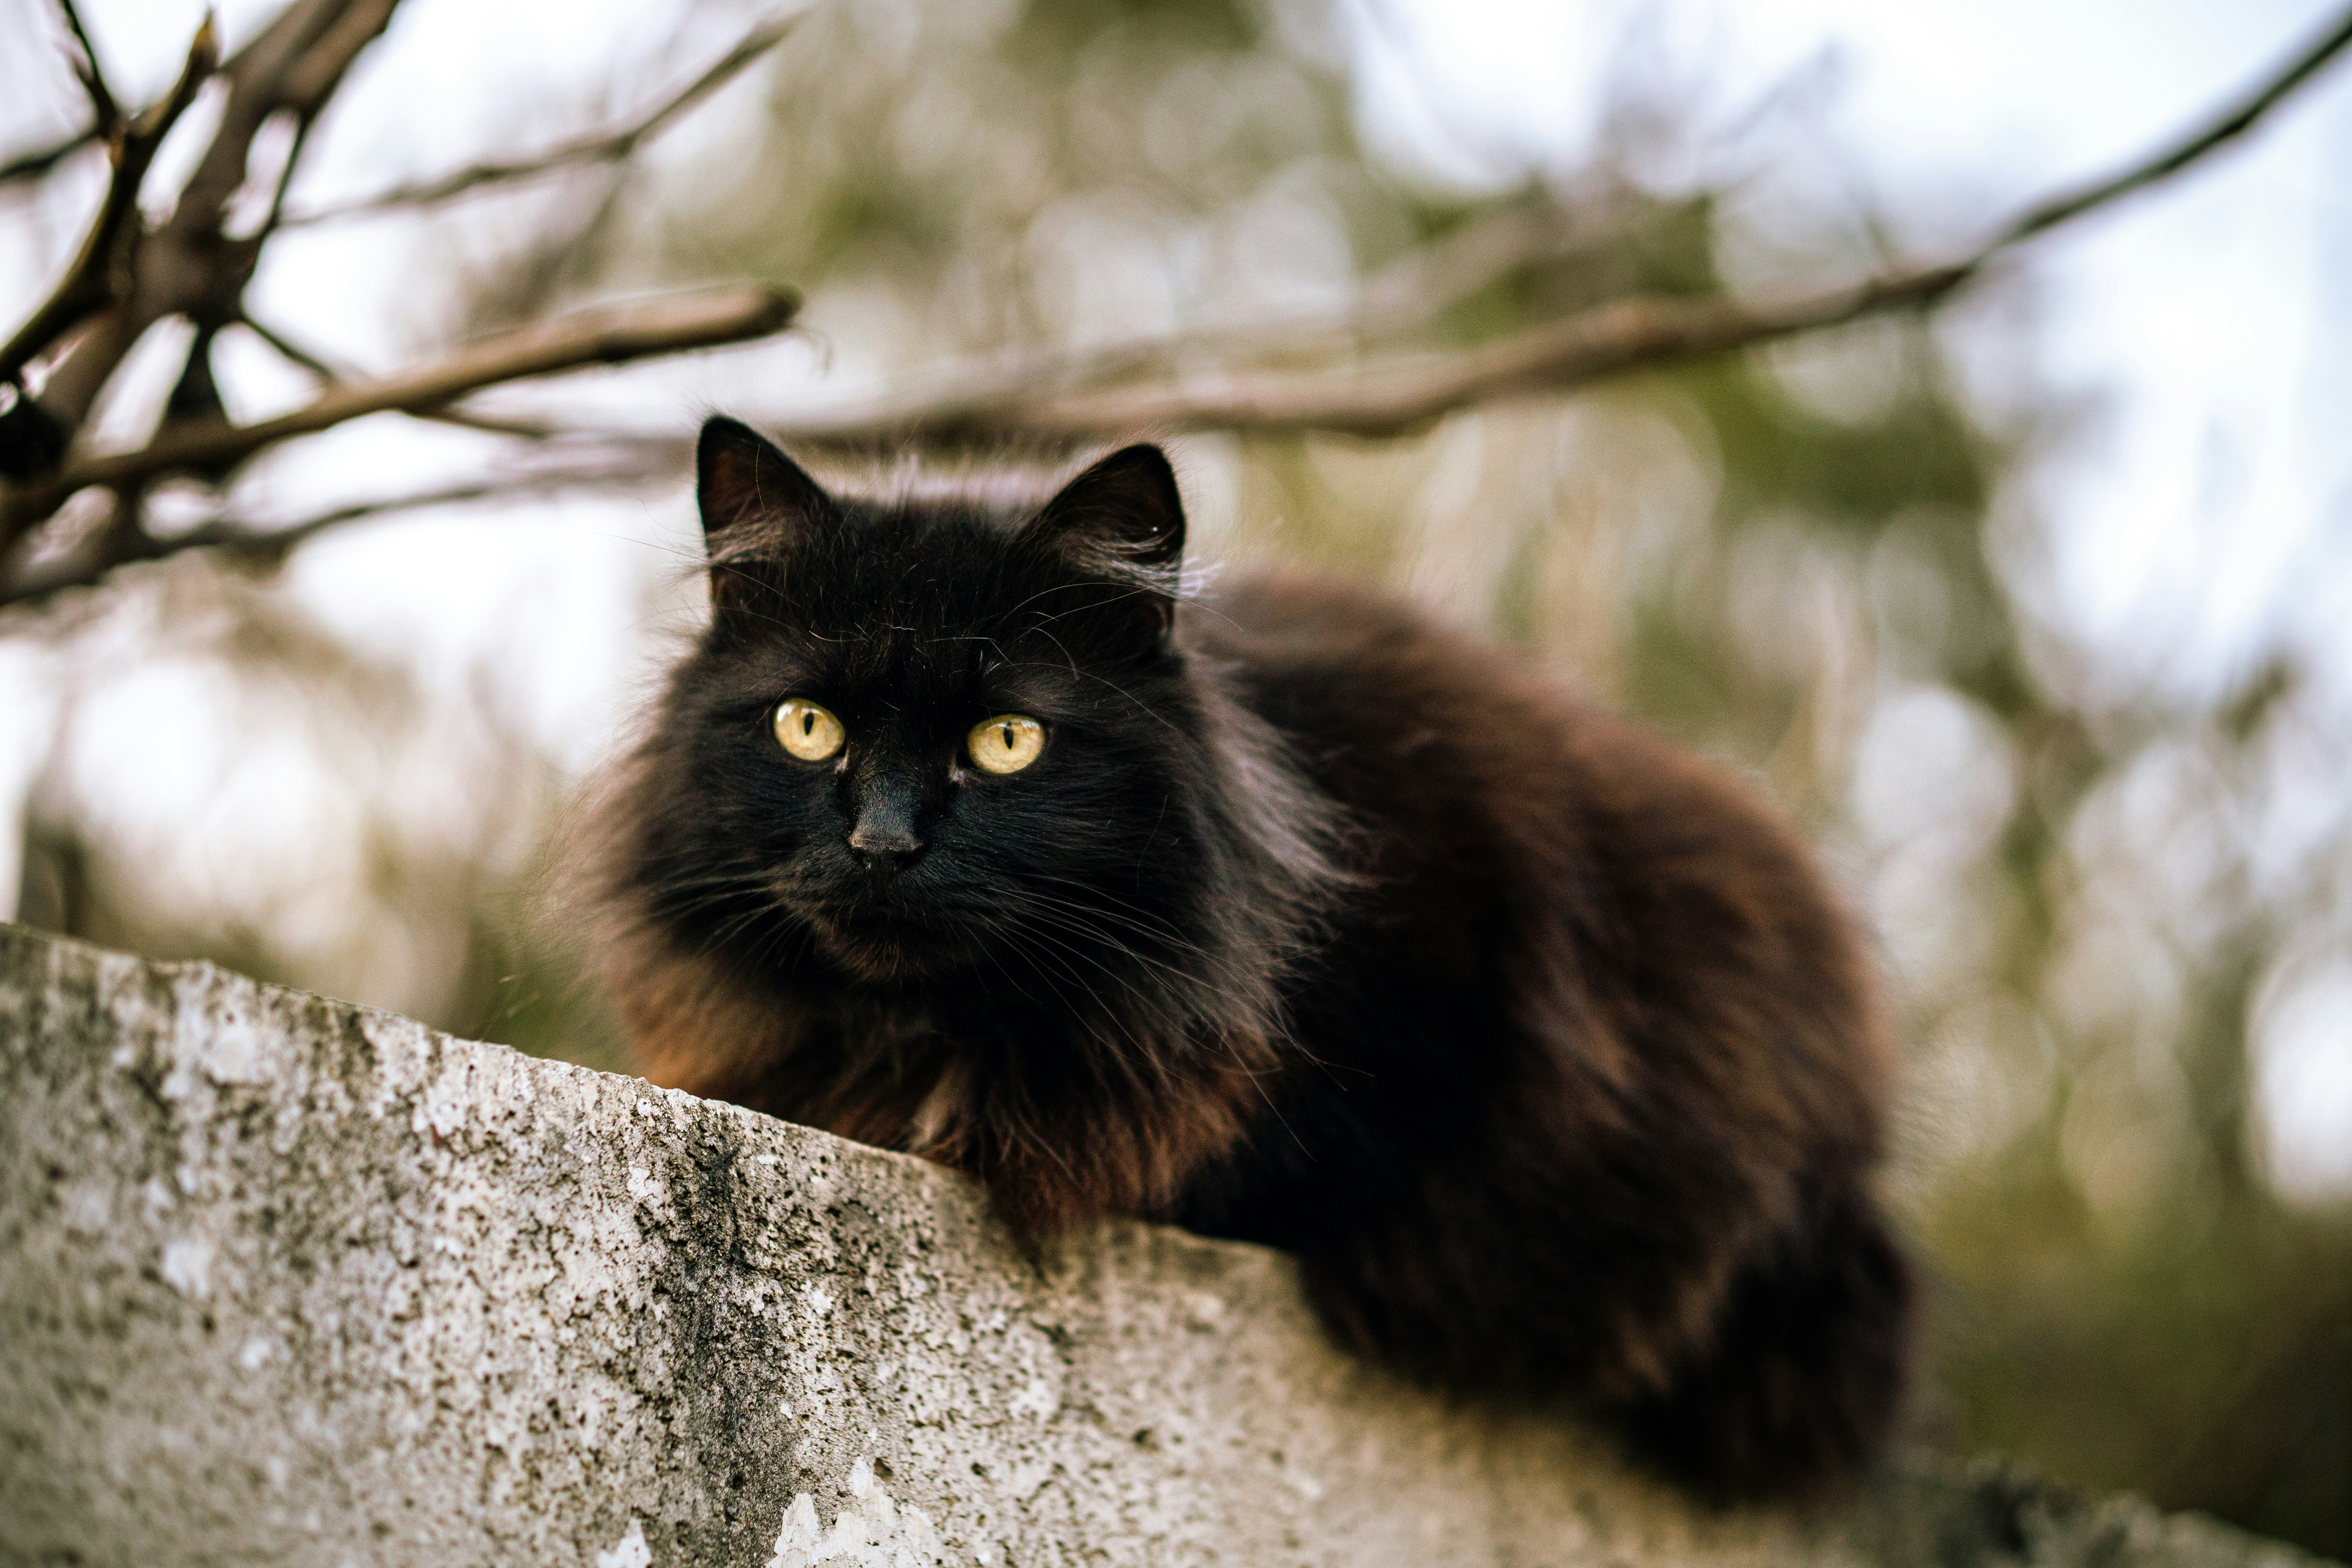
\includegraphics[width=0.5\textwidth]{screenshots/cat.jpeg}
		\caption{Input image}
	\end{figure}
	
	\begin{figure}[H]
		\centering
		
\includegraphics[width=0.9\textwidth]{screenshots/fig_2.png}
		\caption{Multimodal output}
	\end{figure}
	
	\newpage
	\section*{3. Docker Container}
	
	\subsection*{Commands}
	
	\begin{lstlisting}
		docker build -t llm-hw .
		docker run -p 8888:8888 llm-hw
	\end{lstlisting}
	
	\begin{figure}[H]
		\centering
		
\includegraphics[width=0.9\textwidth]{screenshots/fig_3.png}
		\caption{Docker container running}
	\end{figure}
	
	\newpage
	\section*{4. Jupyter Notebook in Docker}
	
	\begin{figure}[H]
		\centering
		
\includegraphics[width=0.9\textwidth]{screenshots/fig_4.png}
		\caption{Jupyter running in browser}
	\end{figure}
	
	\newpage
	\section*{5. Web UI Interaction}
	
	\begin{figure}[H]
		\centering
		
\includegraphics[width=0.9\textwidth]{screenshots/fig_5.png}
		\caption{Open WebUI interacting with model}
	\end{figure}
	
	\section*{Conclusion}
	
	In this assignment, I successfully:
	\begin{itemize}
		\item Ran a local LLM using Ollama
		\item Generated text responses via Python
		\item Used a multimodal model for image understanding
		\item Containerized the application using Docker
		\item Interacted with the model through a web interface
	\end{itemize}
	
	This demonstrates a complete local AI deployment pipeline.
	
\end{document}